% TODO - Ko tad es īsti uztaisīju - lielos un mazos vilcienos?

% TODO - Ko es neuztaisīju!
  
% TODO - No kādām detaļām sastāv mans risinājums?

% TODO - Šeit mēs aprakstam pāris rindkopās to, kamā mēs izpletīsimies nākamajās nodaļās

% Aptuvena ideja: Es uztaisīju aktieru modelī balstītu sistēmu, kas nodrošina centralizētu klientu un aģentu pārvaldību
% ar pieņēmumu, ka gan klienti, gan aģenti jebkurā brīdī varētu atslēgties no sistēmas. Aktieru modelis nosaka, ka sistēma
% ir arī notikumu sistēma, tātad visas izmaiņas sistēmā tiek padotas apkārt izmantojot ziņas jeb vēstules. Notikumu sistēma
% nozīmē, ka ir ļoti viegli klientu un aģentu darbībai paralēli arī žurnalēt to stāvokli piem. datubāzē. Papildus šeit jāpiemin
% kādi tad ir tie aktieri, kas tiek izmantoti šajā sistēmā. 

% Jāpiemin, ko tad tā sistēma īsti nodrošina - ar Scala Play Framework un HTTP REST un Twirl un Slick tā nodrošina biznesa datu CRUD pārvaldību un
% basic auth autentifikāciju, savukārt, ar Scala Play Framework un WebSocket un JSON un aktieriem tā nodrošina vāja reāllaika starpkomunikāciju.  

% Vēl jāpiemin, kāda jēga no šīs CRUD pārvaldības, autentifikācijas un vāja reāllaika komunikāciju. CRUD mums ļauj pārvaldīt lietotājus, dzelžus,
% programmaparatūru. Vājā reāllaika komunikācija ļauj augšupielādēt mums programmatūru dzelžos, tad sūtīt un saņemt informāciju starp klientu un dzelzi, 
% kurā darbinās programmaparatūra, tātad ļauj mums mijiedarboties ar dzelzi. Autentifikācija ļauj pārvaldīt piekļuvi CRUD datiem un
% komunikācijai ar dzelžiem.

% Vēl vajadzētu pieminēt, neskaitot iepriekšminētās salīdzinoši tehniskās detaļas, kā šī sistēma atrisina biznesa problēmu jeb izstrādes procesa
% digitalizāciju. Kā ar šo sistēmu var iesūtīt programmaparatūru, dabūt to dzelzī, mijiedarboties ar programmaparatūru, kas darbinās dzelzī, izmantojot
% "virtuālās saskarnes".  

\section{DIP platforma}

Izstrādātā platforma sastāv no \glslink{server}{servera}, \glslink{agent}{aģentiem}
jeb aparatūras starpniekiem, pašas fiziskās attīstītājrīku aparatūras,
\glslink{client}{klientiem} jeb gala lietotājiem ar komandrindas rīkiem, un
pārvaldības paneļa jeb datu pārvaldības tīmekļa lietotnes. Attēlā
\ref{fig:dipdpd0} redzama 0. līm. datu plūsmas diagramma minētai platformai. 

\begin{figure}[H]
    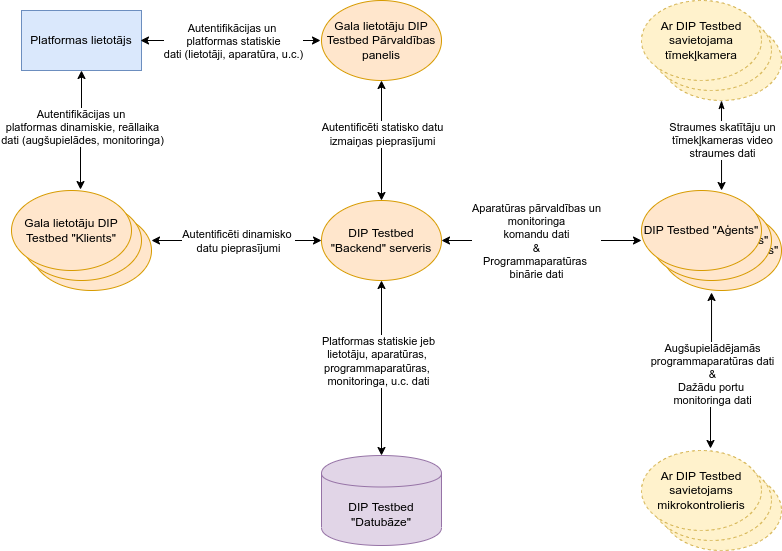
\includegraphics[width=0.7\linewidth]{assets/DPD0.drawio.png}
    \centering
    \caption{DIP platformas 0. līmeņa datu plūsmas diagramma}
    \label{fig:dipdpd0}
\end{figure}

Attēlā \ref{fig:dipdpd0} redzamās apakšsistēmas ir aprakstītas šajā dokumentā
sekojoši. 

Pašā platformas centrā ir centralizēts tīmekļa serveris, kas funkcionē
kā pārvaldības datu avots un platformas lietotāju komunikācijas starpnieks, tā
datu pārvaldības ir aprakstīta nodaļās \ref{sec:usermgmt} un \ref{sec:hwmgmt},
savukārt, tā dalība komunikācijas mehānismos ir aprakstīta \ref{sec:dipactorsystem}.

Nodaļā \ref{sec:dipactorsystem} aprakstītā vājo reāllaika komunikācijas sistēmu,
savukārt, izmanto komandrindas rīki - klients un aģents - lai ļautu lietotājiem
mijiedarboties ar attīstītājrīku aparatūru. Šis mehānisms ir aprakstīts nodaļā
\ref{sec:agentclient}. Un izmantojot šo klienta - aģenta mehānismu, platformā
lietotājam tiek realizētas trīs saskarnes, lai mijiedarbotos ar attīstītājrīku
aparatūru, kuras aprakstītas nodaļās \ref{sec:vinweb}, \ref{sec:vinbytes} un
\ref{sec:vinminos}.

Par šīs platformas, tai skaitā aparatūras laboratoriju, uzstādīšanu un
administrēšanu ir aprakstīts nodaļā \ref{sec:ops}. Par programmaparatūras
izstrādi un testēšanu platformā mazliet aprakstīts nodaļā \ref{sec:usage}. Par
šī darba veikumu un tvērumu aprakstīts nākamajā nodaļā \ref{sec:scope}.

\section{Darba tvērums}
\label{sec:scope}

Darba ietvaros tika izstrādāta vāja reāllaika komunikācijas platforma, kas
nodrošina 1) iespēju reģistrēt un uzskaitīt, pārvaldīt fizisku attīstītājrīku
vai mikrokontrolieru aparatūru, 2) veikt programmaparatūras augšupielādi
aparatūrā, 3) mijiedarboties ar aparatūru, izmantojot vizuālu saskarni, kas
līdzinās noklusētajai aparatūrā fiziski pieejamajai saskarnei, 4) ierobežoti
testēt aparatūras funkcionalitāti. Papildus platforma tika arī testēšanas
nolūkiem izveidota publiskā mākoņpakalpojumu serverī, kas aprakstīts avota koda
repozitorijā un nodaļā \ref{sec:ops}. \cite{VeinbahsKrisjanisTestbed}
\cite{VeinbahsKrisjanisProduction}

Šis darbs izstrādāts atvērti - platformas pirmkods un šī dokumenta pirmkods ir
publiski pieejams GitHub platformā brīvai apskatei un izmantošanai.
\cite{VeinbahsKrisjanisTestbed} \cite{VeinbahsKrisjanisThesis}.

\begin{table}[H]
    \begin{tabular}{ |p{3cm}|p{3cm}|p{3cm}|p{3cm}|p{3cm}| }
    \hline
    Programmēšanas valoda&Faili&Tukšās rindiņas&Komentāru rindiņas&Koda rindiņas\\
    \hline
    Python & 101 & 1551 & 717 & 7424\\
    Scala & 101 & 593 & 120 & 4088\\
    Verilog & 34 & 409 & 676 & 2496\\
    HTML & 11 & 3 & 0 & 492\\
    Bourne Shell & 17 & 91 & 85 & 378\\
    make & 2 & 36 & 30 & 80\\
    SQL & 2 & 33 & 28 & 70\\
    XML & 1 & 14 & 8 & 40\\
    YAML & 2 & 0 & 1 & 33\\
    C++ & 1 & 4 & 14 & 14\\
    \hhline{|=|=|=|=|=|}
    Kopā & 272 & 2734 & 1679 & 15115\\
    \hline
    \end{tabular}
    \centering
    \captionsetup{justification=centering}
    \caption{Koda rindiņu skaita analīze projekta pirmkodā}
    \label{table:cloc}
\end{table}

Aptuvenai sapratnei par izstrādāto koda apjomu, projekta pirmkodā tika izpildīts
koda rindiņu analīzes rīks \cite{AlDanialCloc}, kura rezultāti redzami gan projekta
pirmkoda versiju kontroles repozitorijā \cite{VeinbahsKrisjanisTestbed}, gan tabulā
\ref{table:cloc}.

Platformas pamata funkcionalitāte, lai lietotājs augšupielādētu programmatūru un
veiktu baitu līmeņa datu apmaiņu ar aparatūru, tika realizēta kursa darba laikā.

Bakalaura darba laikā, 1) platformai tika pievienota autentifikācija, 2)
izstrādāts pārvaldības panelis, 3) pārrakstīts klients no tīras grafiskas
saskarnes par termināļa grafisko saskarni, 4) pārrakstīta klienta virtuālā
saskarne kā notikumu sistēma nevis nestrukturizēts kods, 5) izplānota un
realizēta virtuālā saskarne MinOS formālā protokolā, klientā un attīstītājrīkā,
6) tika dokumentēta sistēmas darbība un arhitektūra, tai skaitā arī šī dokumenta
izstrāde.

\section{Statisku datu pārvaldība}
\label{sec:staticdata}

Šī platforma pamatā sastāv no reāllaika datu starpniecības un statisku datu
pārvaldības. Par statiskajiem datiem tiek uzskatīti tādi dati, kurus lietotājs
nemaina izmantojot vājā reāllaika komunikācijas kanālus, kas aprakstīti sadaļā
\ref{sec:dipactorsystem}. 

\begin{figure}[H]
    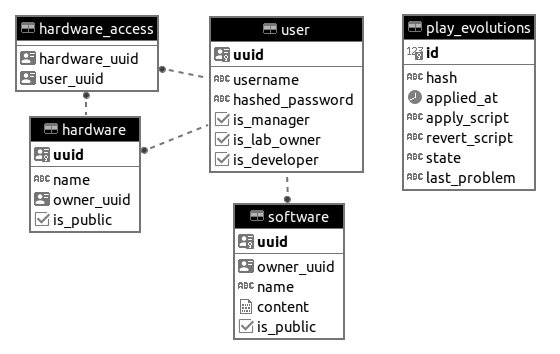
\includegraphics[width=0.7\linewidth]{assets/physical-er-diagram-gray.png}
    \centering
    \caption{Platformas fiziskā līmeņa datubāzes relāciju diagramma.}
    \label{fig:staticdata}
\end{figure}

Attēlā \ref{fig:staticdata} redzama platformas izstrādes laikā izveidotā
datubāzes fiziskā līmeņa relāciju diagramma, kurā redzamas tabulas lietotājiem
"user", programmaparatūrai "software", aparatūrai "hardware" un aparatūras
piekļuvei "hardware\_access", kā arī papildus tabula datubāzes migrāciju
vēstures pārvaldībai "play\_evolutions", kas ir noklusēts tabulas nosaukums
projektā izmantotajam Scala programmēšanas valodas tīmekļa lapu izstrādes
ietvaram "Play Framework".

Lielākoties visām biznesa loģikas entītijām ir piesaistīts \gls{uuid}
identifikators "uuid" un nosaukums "name", papildus dažām entītijām ir dažādi
piekļuves dati formātā "is\_*", programmaparatūrai ir arī tās saturs "content"
un lietotājam ir paroles ar jaucējvērtību datiem "hashed\_password".

Programmaparatūras tabulu varētu arī saukt "firmware", taču platformas izstrādes
laikā tika eksperimentēts platformā arī reģistrēt ne tikai attīstītājrīku
aparatūru, bet arī programmējamus mikrokontrolierus, kuros augšupielādē
programmatūru.

Darba ietvaros tika arī apsvērta tabula "hardware\_messages", lai glabātu vēsturi
par notikušo vājā reāllaika komunikāciju, taču laika ierobežojumu dēļ šī
funkcionalitāte netika realizēta, jo nebija kritiska platformas
funkcionētspējai.

\section{Lietotāju pārvaldības realizācija}
\label{sec:usermgmt}

Lietotāju uzskaitei izmantota attēlā \ref{fig:staticdata} redzamā tabula "user".
Lietotājam ir iespējamas trīs iespējamas lomas pārvaldnieks "manager",
laboratorijas īpašnieks "lab\_owner" un izstrādātājs "developer", atkarībā no
kuras lietotājam platforma piedēvē attiecīgas tiesības veikt dažādas darbības,
kuras skatāmas tabulā \ref{table:permissions}.

\begin{table}[H]
    \newcounter{counter}
    \newcommand\rownumber{\stepcounter{counter}\arabic{counter}.}
    \begin{tabular}{ |p{1cm}|p{5cm}|p{3cm}|p{6cm}| }
    \hline
    N.p.k.&Darbība&Nepieciešamās tiesības&Papildus nosacījumi \\
    \hline
    \rownumber & Lietotāja bez tiesībām izveide & - & Lietotājvārds nevar būt aizņemts \\
    \hline
    \rownumber & Lietotāju datu uzskaite & is\_manager vai is\_lab\_owner & Jebkurš var lasīt savus datus \\
    \hline
    \rownumber & Lietotāja tiesību maiņa & is\_manager & - \\
    \hline
    \rownumber & Programmaparatūras augšupielāde & is\_developer & - \\
    \hline
    \rownumber & Programmaparatūras piekļuve & is\_developer vai is\_manager & Jebkurš var lasīt savu vai publicētu (is\_public) programmaparatūru \\
    \hline
    \rownumber & Programmaparatūras publicēšana & is\_manager & - \\
    \hline
    \rownumber & Aparatūras izveide & is\_lab\_owner & - \\
    \hline
    \rownumber & Aparatūras publicēšana & is\_manager vai is\_lab\_owner &
        Pārvaldnieks var publicēt visu, citi tikai savu \\
    \hline
    \rownumber & Aparatūras uzskaite & is\_manager vai is\_developer, vai
        is\_lab\_owner & Pārvaldnieks var uzskaitīt visu, citi tikai savu vai
        "hardware\_access" tabulā piesaistīto \\
    \hline
    \rownumber & Aparatūras tiesību maiņa & is\_manager vai is\_developer, vai
        is\_lab\_owner & Pārvaldnieks var pārvaldīt visu, citi tikai savu \\
    \hline
    \end{tabular}
    \centering
    \captionsetup{justification=centering}
    \caption{Lietotāju tiesības un pieejamās darbības}
    \label{table:permissions}
\end{table}

Platformā projekta programmatūras konfigurācijā ir konfigurējams administratora
lietotājs ar visām trīs iepriekšminētajām tiesībām, lai izveidotu sākotnējos
pārvaldības lietotājus.

Platformā lietotājus un to piekļuves datus var konfigurēt no
\glslink{mgmtpanel}{pārvaldības paneļa}, kas ir atšķirīgi no pārējām platformas
darbībām, kas lielākoties norit komandu rindā jeb terminālī, jo šos datus
pārsvarā pārvalda pasniedzējs vai laboratorijas īpašnieks, kuram visvieglāk būtu
no jebkura datora atvērt pārlūku un veikt šīs darbības. Savukārt, izstrādātājam,
kas pārsvarā savu darbu veic komandurindā, lielākā daļa darbības ir pieejamas
izmantojot komandu rindas rīku jeb \glslink{client}{klientu}. Skats no
pārvaldības paneļa lietotāju sadaļas skatāms attēlā \ref{fig:mgmtpanelusr}.

\begin{figure}[H]
    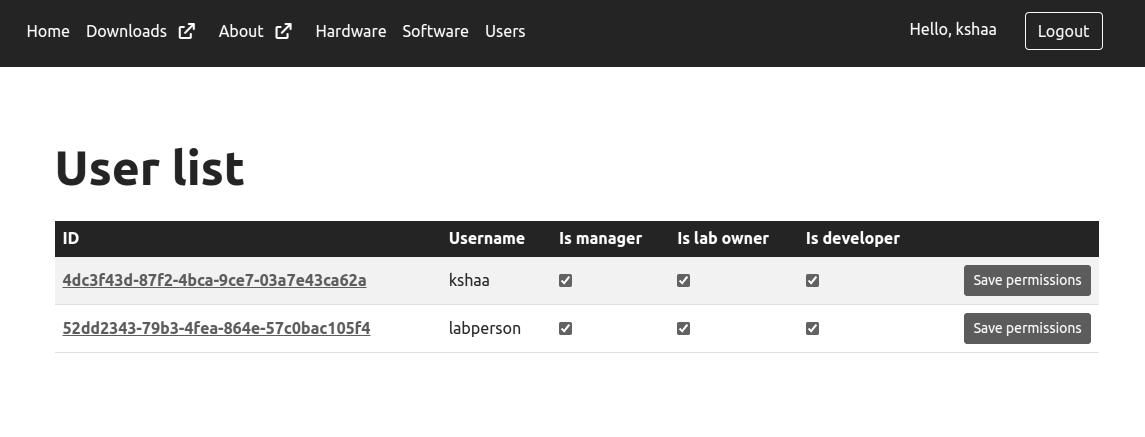
\includegraphics[width=0.9\linewidth]{assets/mgmt-panel-usr-gray.png}
    \centering
    \caption{Platformas pārvaldības paneļa lietotāju pārvaldības skats.}
    \label{fig:mgmtpanelusr}
\end{figure}

\section{Notikumu sistēmas algoritma realizācija}
\label{sec:dipactorsystem}

1. HTTP REST - Biznesa entītiju pārvaldība centrālajā serverī
2. HTTP WebSocket - Vāja reāllaika komunikācija starp centrālo serveri un klientiem/aģentiem
3. Akka - Centrālā servera aktieru vāja reāllaika komunikācija

Agent JSON protocol

Notikumu dzinējs ar blakusefektiem - notikumu sistēmas realizācija gan klientā, gan aģentā, gan serverī.

Actor model (every actor defines its inputs)

Message passing.

Event engines.

Event sourcing.

Purity and side-effects.

\section{Aparatūras pārvaldības realizācija}
\label{sec:hwmgmt}

Komandrindas rīki, Scala, Play, JSON API, header auth.

\section{Aģenti un klienti un to starpkomunikācija}
\label{sec:agentclient}

Kā strādā aģenti, kā tie klausās komandas no platformas, kā tie veic programmēšanu,
kā tie uztur virtuālās saskarnes komunikācijas?

Kā strādā klienti? Kā tie sūta CRUD izmaiņas? Kā tie sūta aģentiem komandas? Kā tie
komunicē ar aģentu programmaparatūru izmantojot seriālo portu.

UART, Virtual Interfaces (webcam, serial connection)

\section{Virtuālā saskarne "tīmekļkamera"}
\label{sec:vinweb}

Visi veidi kā es mēģināju realizēt tīmekļkameras virtuālo saskarni.

Cik labi tas strādā?

Kā to varētu izdarīt vēl labāk?

Īsumā - OGG video streaming

\section{Virtuālās saskarnes "hexbytes" un "buttonleds"}
\label{sec:vinbytes}

5. USB serial - Izmantots komunikācijai starp aģentu un dzelzi


Apraksts dažādu veidu 1-pret-1 baitu ziņapmaiņas virtuālajām saskarnēm.

Ko ar tām var panākt?

Ko ar tām nevar panākt?

\section{Virtuālā saskarne "MinOS"}
\label{sec:vinminos}

MinOS ir virtuāla saskarne, lai mijiedarbotos ar attīstītājrīku aparatūru, kas
ir realizēta kā termināļa grafiskā saskarne, kas redzama attēlā
\ref{fig:minosgui}, taču vizuāli tā līdzinās tai pašai saskarnei, kas pieejama
uz Anvyl attīstītājrīka fiziski, kas redzama attēlā \ref{fig:anvyl}. 

Skatoties attēla \ref{fig:minosgui} saskarnē, ir redzams 8x8 RGB displejs (skat.
kreiso daļu), 8 sarkanas LED gaismas (skat. labās puses 1. rindu), 8 sarkani LED
slēdži (skat. labās puses 2. rindu), 3x8 pelēkas spiedpogas (skat. labās puses
3.-5. rindu), teksta lauki (skat. labās puses 6.-7. rindu). 

\begin{figure}[H]
    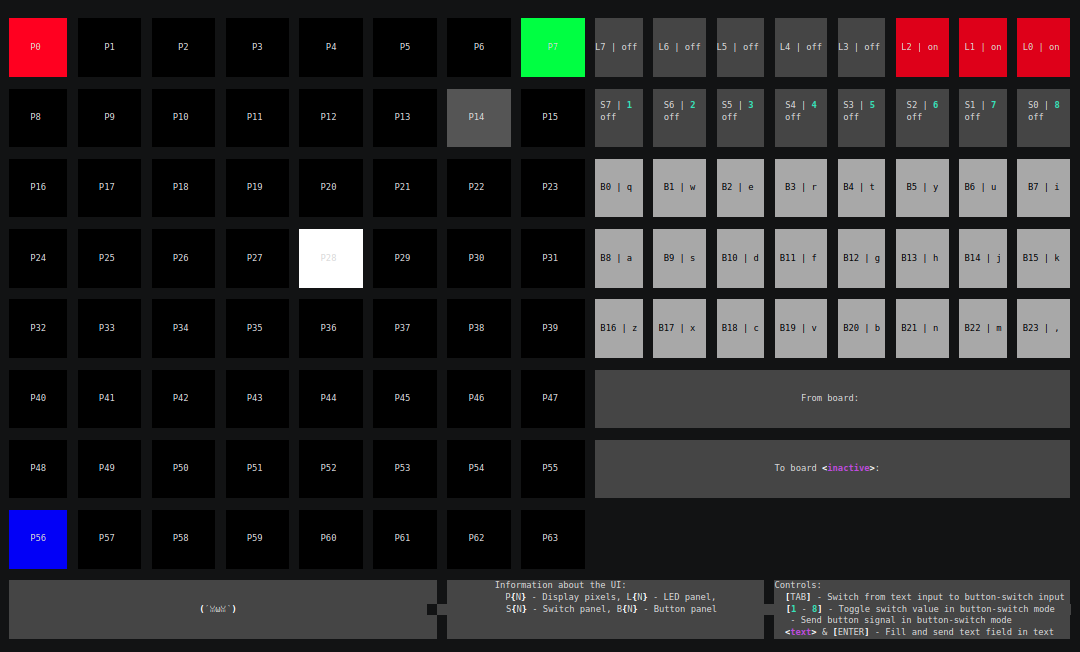
\includegraphics[width=0.7\linewidth]{assets/min-os-execution.png}
    \centering
    \caption{MinOS termināļa grafiskā saskarne.}
    \label{fig:minosgui}
\end{figure}

\begin{figure}[H]
    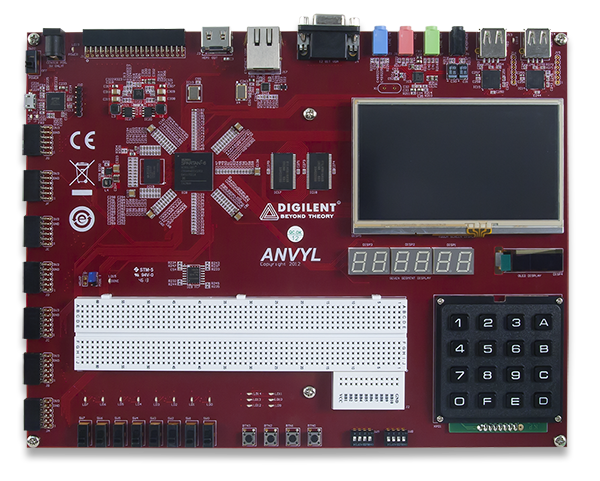
\includegraphics[width=0.7\linewidth]{assets/anvyl.png}
    \centering
    \caption{Anvyl attīstītājrīks.}
    \label{fig:anvyl}
\end{figure}

Lai realizētu MinOS virtuālo saskarni tika izplānots komunikāciju protokols
starp aģentu un klientu. Protokols tika formāli definēts, izstrādājot BNF
formāta sintaksi, kuru iespējams apskatīt pielikumā \ref{att:minosbnf}. Ņemot
vērā, ka vēlamais protokols ir binārs, tad BNF formāts definē baitus kā
heksidecimālu ciparu pārus tātad "0x??".

\ref{lst:minosledchunk}

\begin{lstlisting}[caption={MinOS LED gaismu pakete},label={lst:minosledchunk},captionpos=b]
    0x00 0x02 0xFF 0x00 0x01 
\end{lstlisting}

Pielikums attēls: TUI saskarne https://github.com/kshaa/dip-testbed-dist/blob/master/docs/assets/UHuU1Ur8e0CgoTmsm5khLuOJH.png

Pielikums attēls: 

Ko ar šo saskarni var panākt?

Ko ar šo saskarni nevar panākt?

\section{Infrastruktūras pārvaldība}
\label{sec:ops}

Kā laboratorijas īpašnieki pieslēdz savus dzelžus platformai?

Kā klienti pieslēdzas sistēmai un gūst iespēju izmantot dzelžus?

Kā izstrādātājs jeb darba autors jeb es automatizē versionēšanu, artefaktu pārvaldību?

Docker cross-platform w/ buildx i.e. buildkit

Board management w/ Ansible

CICD deployment procesi

\section{Testēšana un uzturēšana}
\label{sec:usage}

Šo es praktiski neesmu paspējis izdarīt, bet šis būtu interesanti:

Waveform recordings

WASM testing

Ko reāli varētu izdarīt (drīzumā uzkodēšu, šim vajadzētu būt ātri):

MinOS request and response
